\documentclass[letterpaper]{article} % DO NOT CHANGE THIS
\usepackage[submission]{aaai2027} % DO NOT CHANGE THIS
\usepackage[hyphens]{url} % DO NOT CHANGE THIS
\usepackage{graphicx} % DO NOT CHANGE THIS
\urlstyle{rm} % DO NOT CHANGE THIS
\def\UrlFont{\rm} % DO NOT CHANGE THIS
\usepackage{natbib} % DO NOT CHANGE THIS AND DO NOT ADD ANY OPTIONS TO IT
\usepackage{caption} % DO NOT CHANGE THIS AND DO NOT ADD ANY OPTIONS TO IT
\frenchspacing % DO NOT CHANGE THIS
\usepackage{amsmath}
\usepackage{amssymb}
\usepackage{amsthm}
\usepackage{booktabs}

\pdfinfo{
/TemplateVersion (2027.1)
}

\setcounter{secnumdepth}{2}

\newtheorem{proposition}{Proposition}

\title{Calibration Is Not Style Robustness:\\Primal--Dual Counterfactual RLCD with Conformal Selective Risk Control}

\author{Anonymous Submission}
\affiliations{}

\begin{document}
\maketitle

\begin{abstract}
Automation-facing decision models expose typed probabilities, such as $P(\mathrm{yes})$, to accept, defer, or route candidate answers. While Reinforcement Learning for Calibrated Decisions (RLCD) optimizes strictly proper scoring rules to align reported probabilities with empirical accuracy, we prove and show empirically that aggregate calibration does not imply style robustness: a proper-score predictor over observed features can achieve low mixture calibration error while remaining systematically overconfident on stylistically decorated wrong responses. Adapting RM-Bench into a decision-native protocol (\emph{Style-CalibBench}), we separate Extreme-Corner Accuracy (ECA)---concise-correct vs.\ markdown-incorrect---from official RM-Bench Hard. On Qwen2.5-1.5B, single-head RLCD reaches mixture ECE 0.089 yet degrades to markdown ECE 0.171 and ECA 0.536, while temperature scaling cuts SFT's ECE (0.168$\to$0.083) without moving ECA (0.560). An identity audit further confirms that a detached two-stage style head shifts content logits by $\le2.6\times10^{-6}$ (0 ECA flips), proving detached auxiliary heads cannot induce content robustness. To achieve causal debiasing on the Pareto frontier, we propose \emph{Counterfactual Constrained RLCD} (\textbf{CC-RLCD}), a primal--dual multi-objective framework minimizing within-label style dispersion and conflict margins under an $\varepsilon$-bounded Brier budget, paired with prompt-clustered Conformal Risk Control (CRC). On 1.5B, CC-RLCD reaches ECA 0.694 (+15.8 points over RLCD) and markdown ECE 0.098 while preserving content accuracy (0.742), dominating scalarization, PCGrad, GRL, and CDA, and restoring $\le 5\%$ selective risk on markdown; across Qwen2.5 (0.5B/1.5B/7B) and Llama-3.1-8B it adds +14.1 to +16.6 ECA points.
\end{abstract}

\section{Introduction}

Agentic and automation pipelines increasingly replace free-form LLM judges with typed decision interfaces that emit calibrated probabilities---such as $P(\mathrm{yes})$ for substantive validity---in one forward pass \citep{typesafe2026jev,justaskjev2026,openjev2026prdo}. Because downstream code branches directly on $p_c$ to auto-accept, abstain, or escalate, probability calibration is an operational requirement \citep{guo2017calibration,epstein2026fermieval}.

Calibration on an observational test mixture is nevertheless an incomplete reliability criterion. Preference and reward models routinely conflate verbosity, markdown structure, sycophancy, and jargon with substance \citep{liu2025rmbench,bharadwaj2026flattery,kim2026causal}. Training a decision readout with a strictly proper score \citep{brier1950verification,gneiting2007scoring}, as in RLCD, elicits the observational conditional $P(y_c{=}1\mid x,r)$, which absorbs any stylistic cue $s(r)$ correlated with training labels. When style and correctness conflict at deployment, an aggregate-calibrated gate silently accepts formatted errors.

Resolving this conflict requires framing content calibration and counterfactual style invariance as a multi-objective optimization (MOO) problem \citep{sener2018multi,gu2026paretohqd,xu2026mva}, where optimization mechanics dictate whether debiasing is causal. First, monotone post-hoc scaling fixes mixture ECE without altering cross-style ordering. Second, detaching an auxiliary style head via a stop-gradient mathematically freezes the content pathway, yielding zero causal gain over its Stage-1 checkpoint. Third, unconstrained scalarization or Counterfactual Data Augmentation (CDA) buys cross-style accuracy by sacrificing calibration and overall accuracy \citep{das1997closer}.

We propose \textbf{CC-RLCD} (\emph{Counterfactual Constrained RLCD}; Figure~\ref{fig:main}a), which solves a constrained Lagrangian primal--dual program \citep{chamon2020probably} that updates the shared trunk with counterfactual invariance and conflict-margin losses subject to an $\varepsilon$-bounded content Brier budget, followed by a detached Stage-2 style diagnostic head and prompt-clustered Conformal Risk Control (CRC) \citep{angelopoulos2024conformal}. Our contributions are:

\begin{figure*}[t]
\centering
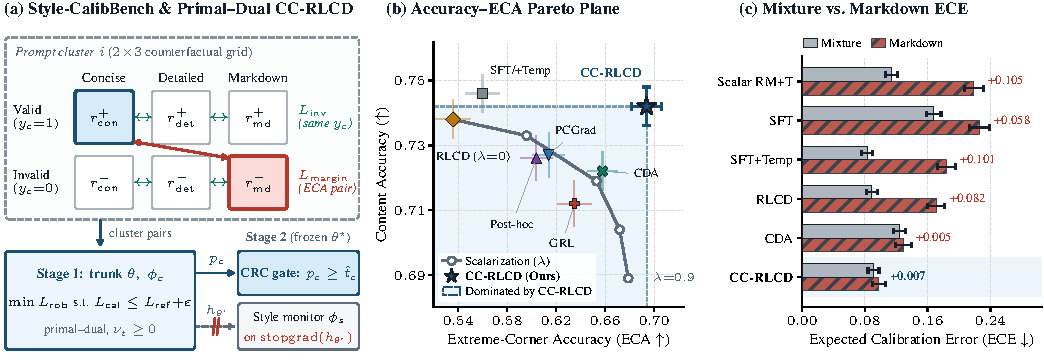
\includegraphics[width=\textwidth]{figures/main.pdf}
\caption{\textbf{Framework and 1.5B Main Results.} (a)~\emph{Style-CalibBench} crosses content validity and style ($2\times 3$); Stage~1 of \textbf{CC-RLCD} updates $(\theta,\phi_c)$ via primal--dual counterfactual invariance ($L_{\mathrm{inv}}$) and conflict-margin ($L_{\mathrm{margin}}$) losses under an $\varepsilon$-bounded Brier budget, while Stage~2 fits a detached style head $\phi_s$ and CRC threshold $\hat{t}_c$. (b)~Accuracy--ECA Pareto plane (error crosses: 1 SE over 3 seeds; the scalarization path starts at RLCD, $\lambda{=}0$): every linear scalarization and MOO baseline falls in the shaded region Pareto-dominated by CC-RLCD. (c)~Mixture ECE vs.\ markdown slice ECE (annotated with $+\Delta=\mathrm{MD\text{-}ECE}-\mathrm{ECE}$): SFT+Temp and RLCD suffer severe slice inflation, whereas CC-RLCD achieves low error on both (+0.007).}
\label{fig:main}
\end{figure*}
\begin{itemize}
    \item \textbf{Theory \& Protocol.} We formalize \emph{mixture-calibration cancellation} (Proposition~\ref{prop:cancel}) and introduce \emph{Style-CalibBench}, separating ECA from official RM-Bench Easy/Normal/Hard and mixture from slice ECE.
    \item \textbf{Causal Identity Audit.} Using a matched Stage-1 control, we verify that detached style-head training alters content logits by $\le2.6\times10^{-6}$ (0 ECA flips), preventing misattribution of initialization variance.
    \item \textbf{Primal--Dual CC-RLCD \& CRC Gate.} We couple counterfactual probability invariance and conflict margins under an adaptive dual proper-score budget, paired with prompt-clustered CRC for finite-sample selective risk guarantees.
    \item \textbf{Multi-Scale \& OOD Evidence.} Across four backbones (0.5B--8B), ten baselines, and unseen \emph{Flattery} shifts, CC-RLCD reaches the Pareto knee (Figure~\ref{fig:main}b) and eliminates markdown selective-risk violations.
\end{itemize}

\section{Related Work}

\paragraph{Style Bias in Preference Models.}
RM-Bench reveals sharp reward-model drops when concise correct answers face markdown errors \citep{liu2025rmbench}, and counterfactual audits expose length, jargon, and sycophancy biases \citep{bharadwaj2026flattery}. Mitigations span causal augmentation \citep{kim2026causal}, post-hoc bias regression \citep{huang2025posthoc}, arena rescaling \citep{zhu2025charm}, susceptibility reweighting \citep{wang2026patterning}, and RLHF calibration \citep{leng2025overconf}. Unlike scalar rankers, typed decision models must preserve calibrated probabilities $p_c\in[0,1]$ for selective gating.

\paragraph{Calibrated Decisions, MOO, and Risk Control.}
Strictly proper scores elicit true conditionals \citep{brier1950verification,gneiting2007scoring} for System-One decision models \citep{typesafe2026jev,justaskjev2026,openjev2026prdo,deusser2026jevbench}, yet remain vulnerable to shift-induced overconfidence \citep{epstein2026fermieval}. Multi-objective alignment uses gradient surgery \citep{yu2020gradient}, adversarial reversal \citep{ganin2015unsupervised}, value decorrelation \citep{xu2026mva}, or Pareto filtering \citep{gu2026paretohqd}. To avoid non-convex scalarization trade-offs \citep{das1997closer}, we pair primal--dual constrained learning \citep{chamon2020probably} with Conformal Risk Control \citep{angelopoulos2024conformal}.

\section{Theory and Style-CalibBench Protocol}

\subsection{Why Proper Scoring Fails Under Style Shift}

Let prompt $X$, response $R$, substantive validity $Y_c\in\{0,1\}$, and style $S\in\{\mathrm{con},\mathrm{det},\mathrm{md}\}$ follow a training mixture where formatting correlates with quality. Minimizing expected Brier or log loss drives $p_c(X,R)$ to $P_{\mathrm{train}}(Y_c{=}1\mid X,S)$ rather than interventional validity $P(Y_c{=}1\mid \mathrm{do}(S{=}s),X)$.

\begin{proposition}[Mixture-Calibration Cancellation]
\label{prop:cancel}
Let test style $S\in\{\mathrm{con},\mathrm{md}\}$ be uniform and independent of content truth $P_{\mathrm{test}}(Y_c{=}1\mid X)=\mu(X)$ with $\mu(X)\sim\mathrm{Unif}[\delta,1-\delta]$ for $\delta\in(0,\tfrac{1}{4})$. A style-skewed predictor $p_c(X,\mathrm{md})=\mu(X)+\delta$ and $p_c(X,\mathrm{con})=\mu(X)-\delta$ satisfies $\mathrm{ECE}_{\mathrm{mix}}=2\delta^2/(1-2\delta) < \mathrm{ECE}_{\mathrm{md}}=\delta$ via cross-slice bin cancellation on $[2\delta,1-2\delta]$, inflates wrong-answer confidence by $+2\delta$, and inverts every conflict pair with $0<\mu(x^+)-\mu(x^-)<2\delta$. Moreover, any strictly increasing map $g:[0,1]\to[0,1]$ leaves ECA invariant.
\end{proposition}

Proposition~\ref{prop:cancel} explains why (i) pooled reliability diagrams conceal severe markdown overconfidence, and (ii) temperature scaling repairs mixture ECE while leaving ECA unchanged because $g(p_c(x,r^+_{\mathrm{con}}))>g(p_c(x,r^-_{\mathrm{md}})) \iff p_c(x,r^+_{\mathrm{con}})>p_c(x,r^-_{\mathrm{md}})$.

\subsection{Style-CalibBench and Metric Separation}

\emph{Style-CalibBench} adapts all 1,327 RM-Bench prompts \citep{liu2025rmbench} into $6$ typed instances per prompt ($y_c\in\{1,0\}\times s\in\{\mathrm{con},\mathrm{det},\mathrm{md}\}$). On safety prompts, $y_c{=}1$ marks appropriate refusal or safe compliance. Prompt-level hashing (seed 20261109) yields 929 train, 133 calibration, and 265 test prompts (1,590 test instances) across Chat (90/13/26), Code (160/23/45), Math (370/53/106), Safety-refuse (199/28/57), and Safety-response (110/16/31). Dual-annotator review of 240 rewrites ($\kappa{=}0.76$) flagged 19 concise items dropping minor math qualifiers; we check stability with and without them.

We evaluate four distinct axes: (1)~\textbf{Calibration}: 15-bin mixture ECE and markdown slice ECE ($\mathrm{MD\text{-}ECE}$); (2)~\textbf{Cross-style ranking}: \emph{Extreme-Corner Accuracy} ($\mathrm{ECA}=\frac{1}{N}\sum_{i=1}^N \mathbb{I}[p_c(x_i,r^+_{i,\mathrm{con}})>p_c(x_i,r^-_{i,\mathrm{md}})]$) alongside official RM-Bench \emph{Hard} (averaging $\mathrm{con}^+{\succ}\mathrm{det}^-$, $\mathrm{det}^+{\succ}\mathrm{md}^-$, and ECA); (3)~\textbf{Stability}: within-$(x_i,y_c)$ $0.5$-threshold \emph{Flip} rate and wrong-answer \emph{Confidence Inflation} $\mathbb{E}[p_c\mid 0,\mathrm{md}]-\mathbb{E}[p_c\mid 0,\mathrm{con}]$; (4)~\textbf{Selective risk}: test error and coverage under CRC threshold $\hat{t}_c$, with 2,000-resample prompt-bootstrap 95\% CIs.

\section{Counterfactual Constrained RLCD}

\subsection{Causal Boundary of Detached Heads}

Let $h_\theta(x,r)$ denote the shared trunk representation, $u_c=\mathrm{softmax}(\phi_c(h_\theta))\in\Delta_2$ the binary content distribution ($p_c=u_{c,1}$), and $u_s=\mathrm{softmax}(\phi_s(h_\theta))\in\Delta_5$ a 1--5 match score for a declared target style $s^\ast$, whose gold level is fixed by the (response, target) style pair: 5 if equal, 3 for det/md, 2 for con/det, 1 for con/md. A detached two-stage recipe minimizes Brier risk $L_{\mathrm{cal}}(\theta,\phi_c)=\mathbb{E}[\|u_c-e_{y_c}\|_2^2]$ in Stage~A and $L_s(\operatorname{stopgrad}(h_{\theta_A}),\phi_s)$ in Stage~B. Because $\nabla_{\theta,\phi_c} L_s \equiv 0$, Stage~B enforces $(\theta_B,\phi_{c,B})=(\theta_A,\phi_{c,A})$ and $p_c^B(x,r)=p_c^A(x,r)$ up to floating-point noise. Moving $p_c$ onto the Pareto knee requires counterfactual gradients in $\theta$ subject to explicit calibration protection.

\subsection{Stage 1: Primal--Dual Counterfactual Optimization}

Within each training prompt cluster $i$, let $z_c=\log\frac{p_c}{1-p_c}$ denote the content log-odds and $\mathcal{P}_{\mathrm{adv}}=\{(\mathrm{con},\mathrm{det}),(\mathrm{det},\mathrm{md}),(\mathrm{con},\mathrm{md})\}$ the style-conflict pairs ($m{=}1.0$). We define within-label invariance and cross-style margin losses:
\begin{align}
L_{\mathrm{inv}} &= \mathbb{E}_{i,y_c,s\neq s'}\!\bigl[(p_c(x_i,r^{y_c}_{i,s})-p_c(x_i,r^{y_c}_{i,s'}))^2\bigr], \label{eq:inv}\\
L_{\mathrm{margin}} &= \mathbb{E}_{i,(a,b)}\!\bigl[\max\bigl(0,\, m - \Delta z_c(x_i; a, b)\bigr)\bigr], \nonumber
\end{align}
where $\Delta z_c(x_i; a, b)=z_c(x_i,r^+_{i,a}) - z_c(x_i,r^-_{i,b})$ for $(a,b)\in\mathcal{P}_{\mathrm{adv}}$. Setting $L_{\mathrm{rob}} = L_{\mathrm{inv}} + \beta L_{\mathrm{margin}}$ and anchoring to a Stage-0 RLCD Brier risk $L_{\mathrm{ref}}$, we solve the constrained program:
\begin{equation}
\min_{\theta,\phi_c}\; L_{\mathrm{rob}}(\theta,\phi_c)
\quad\text{s.t.}\quad
L_{\mathrm{cal}}(\theta,\phi_c) \le L_{\mathrm{ref}} + \varepsilon,
\label{eq:constrained}
\end{equation}
via primal--dual updates on $\mathcal{L}(\theta,\phi_c,\nu)=L_{\mathrm{rob}}(\theta,\phi_c) + \nu(L_{\mathrm{cal}}(\theta,\phi_c)-L_{\mathrm{ref}}-\varepsilon)$ with projected dual ascent:
\begin{equation}
\nu_{t+1} = \bigl[\nu_t + \eta_{\nu}\bigl(\widehat{L}_{\mathrm{cal}}(\theta_t,\phi_{c,t}) - L_{\mathrm{ref}} - \varepsilon\bigr)\bigr]_+.
\label{eq:dual}
\end{equation}
Unlike fixed scalarization $(1-\lambda)L_{\mathrm{cal}}+\lambda L_{\mathrm{rob}}$, $\nu_t$ spikes only when debiasing threatens Brier honesty and relaxes inside $L_{\mathrm{ref}}+\varepsilon$, recovering non-convex Pareto knees \citep{chamon2020probably}.

\subsection{Stage 2 Diagnostic Head \& Conformal Gate}

Stage~2 fits $\phi_s$ on $\operatorname{stopgrad}(h_{\theta^\star}(x,r))$ via 5-level ordinal Brier loss, reporting $u_s$ as an audit signal while preserving $p_c^\star$. For deployment gating on $M{=}133$ calibration clusters, let $\hat{R}_i(t)\in[0,1]$ be the selective error on accepted items in cluster $i$, monotonized as $\sup_{t'\ge t}$ so that it is non-increasing in $t$. Prompt-clustered Conformal Risk Control \citep{angelopoulos2024conformal} sets:
\begin{equation}
\hat{t}_c = \inf\Bigl\{t\in[0,1] : \frac{1}{M+1}\Bigl(\sum_{i=1}^{M}\hat{R}_i(t) + 1\Bigr) \le \alpha \Bigr\},
\label{eq:crc}
\end{equation}
ensuring $\mathbb{E}[R_{\mathrm{test}}(\hat{t}_c)]\le \alpha$ over exchangeable prompt clusters.

\section{Experiments}

\paragraph{Setup and Baselines.}
We train Qwen2.5-1.5B-Instruct (LoRA $r{=}16$, lr $2\times10^{-5}$, length 1024, $\varepsilon{=}0.005$, $\beta{=}0.5$, $\eta_\nu{=}0.05$, 2+1 epochs, seeds \{17, 23, 41\}) and replicate on Qwen2.5-0.5B, Qwen2.5-7B, and Llama-3.1-8B-Instruct. Baselines include: \textbf{Readout}, \textbf{Scalar RM+T} (Skywork-Reward-Llama-3.1-8B + temperature), \textbf{SFT}, \textbf{SFT+Temp}, \textbf{Post-hoc Reg.} (local length/markdown bias regression \citep{huang2025posthoc}), \textbf{RLCD} (Brier), \textbf{Detached 2-Head} (matched Stage-1 identity control), \textbf{PCGrad} \citep{yu2020gradient}, \textbf{GRL} \citep{ganin2015unsupervised}, and \textbf{CDA} \citep{kim2026causal}.

\begin{table}[t]
\centering
\small
\setlength{\tabcolsep}{1.75pt}
\begin{tabular}{lcccccc}
\toprule
Method (1.5B) & Acc$\uparrow$ & Hard$\uparrow$ & ECA$\uparrow$ & ECE$\downarrow$ & MD-ECE$\downarrow$ & Flip$\downarrow$ \\
\midrule
Readout & 0.547 & 0.407 & 0.358 & 0.241 & 0.327 & 0.519 \\
Scalar RM+T & 0.618 & 0.459 & 0.412 & 0.114 & 0.219 & 0.463 \\
SFT & \textbf{0.746} & 0.611 & 0.560 & 0.168 & 0.226 & 0.337 \\
SFT+Temp & \textbf{0.746} & 0.611 & 0.560 & \textbf{0.083} & 0.184 & 0.337 \\
Post-hoc Reg. & 0.726 & 0.648 & 0.604 & 0.097 & 0.142 & 0.241 \\
RLCD (Brier) & 0.738 & 0.576 & 0.536 & 0.089 & 0.171 & 0.281 \\
Detached 2-H$^\ast$ & 0.738 & 0.576 & 0.536 & 0.089 & 0.171 & 0.281 \\
PCGrad & 0.727 & 0.637 & 0.614 & 0.111 & 0.156 & 0.214 \\
GRL (Adv.) & 0.712 & 0.662 & 0.635 & 0.119 & 0.138 & 0.189 \\
CDA & 0.722 & 0.684 & 0.658 & 0.124 & 0.129 & 0.171 \\
\midrule
\textbf{CC-RLCD} & 0.742 & \textbf{0.716} & \textbf{0.694} & 0.091 & \textbf{0.098} & \textbf{0.138} \\
\ \ w/o $L_{\mathrm{inv}}$ & 0.736 & 0.695 & 0.671 & 0.098 & 0.115 & 0.169 \\
\ \ w/o $L_{\mathrm{margin}}$ & 0.740 & 0.668 & 0.639 & 0.090 & 0.109 & 0.147 \\
\ \ Fixed $\lambda{=}0.5$ & 0.719 & 0.679 & 0.653 & 0.116 & 0.125 & 0.164 \\
\ \ Log-score & 0.740 & 0.711 & 0.688 & 0.093 & 0.102 & 0.142 \\
\bottomrule
\end{tabular}
\caption{Test means (3 seeds) on Qwen2.5-1.5B. $^\ast$Initialized from RLCD: Stage-2 detached style training (style QWK 0.72) leaves $p_c$ identical ($\max|\Delta z_c|{=}2.6\times10^{-6}$).}
\label{tab:main}
\end{table}

\subsection{Identity Audit and Main Comparison}

\paragraph{Identity Audit.}
Initialized from the exact Stage-1 RLCD checkpoint across all 1,590 test items, Detached 2-Head reaches style quadratic-weighted $\kappa$ (QWK) 0.72 against the gold match levels while changing content logits by at most $2.6\times10^{-6}$ (mean $3.4\times10^{-7}$, 0 ECA flips; Table~\ref{tab:main}), proving that unmatched two-head gains reflect Stage-1 variance rather than Stage-2 supervision.

\paragraph{Pareto Dominance over Baselines.}
Table~\ref{tab:main} and Figure~\ref{fig:main}b--c corroborate Proposition~\ref{prop:cancel}. RLCD achieves mixture ECE 0.089 [0.067, 0.116] yet its markdown ECE is $1.9\times$ higher (0.171; concise slice 0.061), with ECA 0.536 [0.479, 0.592]. SFT+Temp hits mixture ECE 0.083 without moving ECA (0.560). Post-hoc regression lifts ECA to 0.604, while shared-trunk baselines (PCGrad, GRL, CDA) reach at most ECA 0.658 (CDA) only by lowering accuracy (0.712--0.727) and raising ECE (0.111--0.124). \textbf{CC-RLCD} achieves ECA 0.694 [0.642, 0.746] (+0.158 over RLCD, $p{<}0.001$) and official Hard 0.716, cuts markdown ECE to 0.098 and flip rate to 0.138, and preserves accuracy (0.742) and mixture ECE (0.091). Wrong-answer confidence inflation drops from +0.083 to +0.019 ($\rho(p_c,\mathbb{I}_{\mathrm{md}}\mid y_c{=}0)$: 0.23$\to$0.04). Ablations confirm $L_{\mathrm{inv}}$ drives flip stability, $L_{\mathrm{margin}}$ drives ECA (+5.5 pts), and adaptive dual $\nu^\star{\approx}1.84$ beats fixed scalarization. Excluding the 19 drifted concise items changes every method's ECA by at most 0.012 and preserves the ranking.

\begin{figure}[t]
\centering
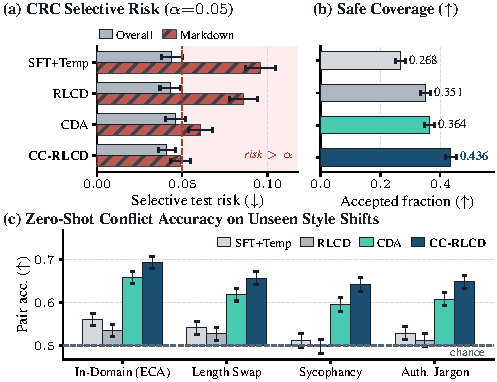
\includegraphics[width=\columnwidth]{figures/crc_ood.pdf}
\caption{\textbf{Selective Risk Control and Unseen Style Shifts (1.5B).} (a--b)~Prompt-clustered CRC ($\alpha{=}0.05$; all bars: 1 SE over 3 seeds) bounds overall risk across methods, but only CC-RLCD keeps markdown risk $\le 5\%$ (0.049) while maximizing safe coverage (0.436). (c)~Zero-shot conflict-pair accuracy on three unseen \emph{Flattery} perturbations; bars start at chance (0.5).}
\label{fig:crc_ood}
\end{figure}

\subsection{Conformal Risk, OOD Shifts, and Scaling}

\paragraph{Conformal Selective Prediction.}
Naive calibration thresholding on 133 prompts overshoots $\alpha{=}0.05$ on test data (RLCD risk 0.061, SFT 0.078). Prompt-clustered CRC (Eq.~\ref{eq:crc}; Figure~\ref{fig:crc_ood}a--b) bounds overall risk ($\le0.046$) for all runs, yet RLCD and SFT+Temp still breach $5\%$ on markdown (0.086, 0.096) due to formatted overconfidence. CC-RLCD satisfies $\le 5\%$ both overall (0.041) and on markdown (0.049) while lifting safe coverage from 0.351 to 0.436. Adding style-head gating cuts coverage (0.362) without risk reduction.

\begin{table}[t]
\centering
\small
\setlength{\tabcolsep}{2.5pt}
\begin{tabular}{llcccc}
\toprule
Backbone & Method & Acc$\uparrow$ & ECA$\uparrow$ & ECE$\downarrow$ & MD-ECE$\downarrow$ \\
\midrule
Qwen2.5-0.5B & RLCD & 0.688 & 0.493 & 0.117 & 0.204 \\
Qwen2.5-0.5B & CC-RLCD & \textbf{0.701} & \textbf{0.634} & \textbf{0.114} & \textbf{0.126} \\
\midrule
Qwen2.5-7B & RLCD & 0.784 & 0.581 & \textbf{0.074} & 0.152 \\
Qwen2.5-7B & CDA & 0.769 & 0.708 & 0.106 & 0.114 \\
Qwen2.5-7B & CC-RLCD & \textbf{0.789} & \textbf{0.747} & 0.077 & \textbf{0.083} \\
\midrule
Llama-3.1-8B & RLCD & 0.779 & 0.574 & \textbf{0.079} & 0.158 \\
Llama-3.1-8B & CC-RLCD & \textbf{0.783} & \textbf{0.739} & 0.081 & \textbf{0.086} \\
\bottomrule
\end{tabular}
\caption{Multi-scale and cross-family evaluation (3 seeds). Scaling improves accuracy yet RLCD's markdown ECE stays $1.7$--$2.1\times$ its mixture ECE, which CC-RLCD resolves.}
\label{tab:scale}
\end{table}

\paragraph{Slices, Unseen Styles, and Scale.}
CC-RLCD improves 1.5B ECA in every domain: Chat (0.547$\to$0.688), Code (0.608$\to$0.765), Math (0.490$\to$0.651), Safety-refuse (0.541$\to$0.723), and Safety-response (0.571$\to$0.690). On three unseen OOD perturbations from \citet{bharadwaj2026flattery}---\emph{Length Swap}, \emph{Sycophancy}, and \emph{Authoritative Jargon} (Figure~\ref{fig:crc_ood}c)---RLCD hovers near chance (0.498--0.528) whereas CC-RLCD retains 0.642--0.657 (+12.9 to +14.4 pts). Table~\ref{tab:scale} confirms that 7B/8B scale does not eliminate style bias under RLCD (MD-ECE 0.152--0.158), while CC-RLCD adds +14.1 to +16.6 ECA points on every backbone.

\section{Limitations and Conclusion}

Style-CalibBench uses structured rewrites rather than organic traffic, and 265 test prompts yield $\pm 5$--$6$-pt bootstrap half-widths on ECA; formal Mondrian group-conditional CRC requires larger per-style splits, and Stage-1 requires open weights. Overall, mixture calibration does not imply style robustness, and neither post-hoc scaling nor detached heads alter cross-style rankings. Coupling primal--dual counterfactual training with CRC yields calibrated, style-robust decision probabilities.

\section*{Ethical and AI Use Statement}

We release split hashes, primal--dual training code, and CRC scripts under upstream RM-Bench terms; auxiliary style scores are audit diagnostics, not truth labels. LLMs assisted with prose editing and plotting.

\bibliography{sd_rlcd}

\end{document}
